\documentclass[conference]{IEEEtran}
\IEEEoverridecommandlockouts

\usepackage[T1]{fontenc}
\usepackage{cite}
\usepackage{amsmath,amssymb}
\usepackage{graphicx}
\usepackage{booktabs}
\usepackage{url}
\usepackage[hidelinks]{hyperref}

\graphicspath{{../docs/diagrams/}{../docs/waveforms/}}

\begin{document}

\title{Design, Verification, and Evaluation of a Four-Lane SIMD Vector Unit in Verilog}

\author{
\IEEEauthorblockN{Shaik Tajuddin}
\IEEEauthorblockA{\textit{2401010436} \\ shaik.tajuddin2024@nst.rishihood.edu.in}
\and
\IEEEauthorblockN{Parthraj Singh Bhati}
\IEEEauthorblockA{\textit{2401010320} \\ parthraj.bhati2024@nst.rishihood.edu.in}
\and
\IEEEauthorblockN{Himanshu Pandey}
\IEEEauthorblockA{\textit{2401020095} \\ himanshu.h2024@nst.rishihood.edu.in}
\and
\IEEEauthorblockN{Jivit Rana}
\IEEEauthorblockA{\textit{2401010202} \\ jivit.rana2024@nst.rishihood.edu.in}
\and
\IEEEauthorblockN{Satya Yadav}
\IEEEauthorblockA{\textit{2401010427} \\ satya.yadav2024@nst.rishihood.edu.in}
}


\maketitle

\begin{abstract}
This project implements a single-cycle, four-lane SIMD vector processor in
Verilog and compares it with a one-lane scalar baseline. The vector processor
uses a 16-bit instruction format, eight 128-bit vector registers, and a
word-addressed vector memory. It executes integer arithmetic, bitwise logic,
comparisons, shifts, vector loads and stores, and halt. Verification used
eight RTL testbenches and an independent Python ISA simulator. In a fixed-seed
regression, all 2,000 generated programs matched the reference model in final
data memory and cycle count. For the addition of two 16-element arrays, the
vector processor used 16 counted cycles and the scalar baseline used 64,
giving a fourfold improvement in elements per cycle. In module-level Yosys
synthesis, the four-lane ALU used 1,012 lookup tables compared with 251 for one
lane. These results quantify cycle efficiency for the tested kernel and the
area cost of lane replication. Whole-core FPGA area and maximum clock
frequency remain unmeasured.
\end{abstract}

\begin{IEEEkeywords}
SIMD, vector processor, Verilog, RTL verification, FPGA synthesis.
\end{IEEEkeywords}

\section{Literature Review}
Flynn's taxonomy classifies machines by instruction and data streams. SIMD
executes a common operation on multiple data elements, allowing workloads
such as elementwise array arithmetic to exploit data-level parallelism
\cite{flynn1966,hennessy2017}. The CRAY-1 illustrates the use of vector registers
to hold operands for operations across multiple elements \cite{russell1978}.
The RISC-V Vector extension supports configurable vector length and masked
execution \cite{riscvvector}. The processor developed here uses a fixed
four-lane configuration to make the effect of parallel execution measurable
with a small instruction set.

Yu, Lemieux, and Eagleston examined configurable FPGA soft vector
processors and the throughput and hardware trade-offs of scaling their
parallelism \cite{yu2008soft}. We use a related design choice by
replicating one ALU module with a Verilog generate loop. Our evaluation
compares a scalar baseline using that same ALU with a four-lane implementation
on a single kernel. The resulting cycle ratio is specific to this prototype,
workload, and memory organization.

\section{Proposed Solution}
\subsection{Architecture and Execution}
The processor issues one instruction per clock without pipelining. The program
counter (PC) selects a 16-bit word from a 64-word instruction ROM. Program
images are loaded from hexadecimal files using \texttt{\$readmemh}, and
unused entries are initialized to \texttt{F000} (HALT). The vector register
file has eight 128-bit registers, two combinational read ports, and one
rising-edge write port. Data memory holds 16 vector words, has a combinational
read port, and commits writes on the rising edge. Fig.~\ref{fig:architecture}
shows the integrated datapath.

\begin{figure}[t]
\centering
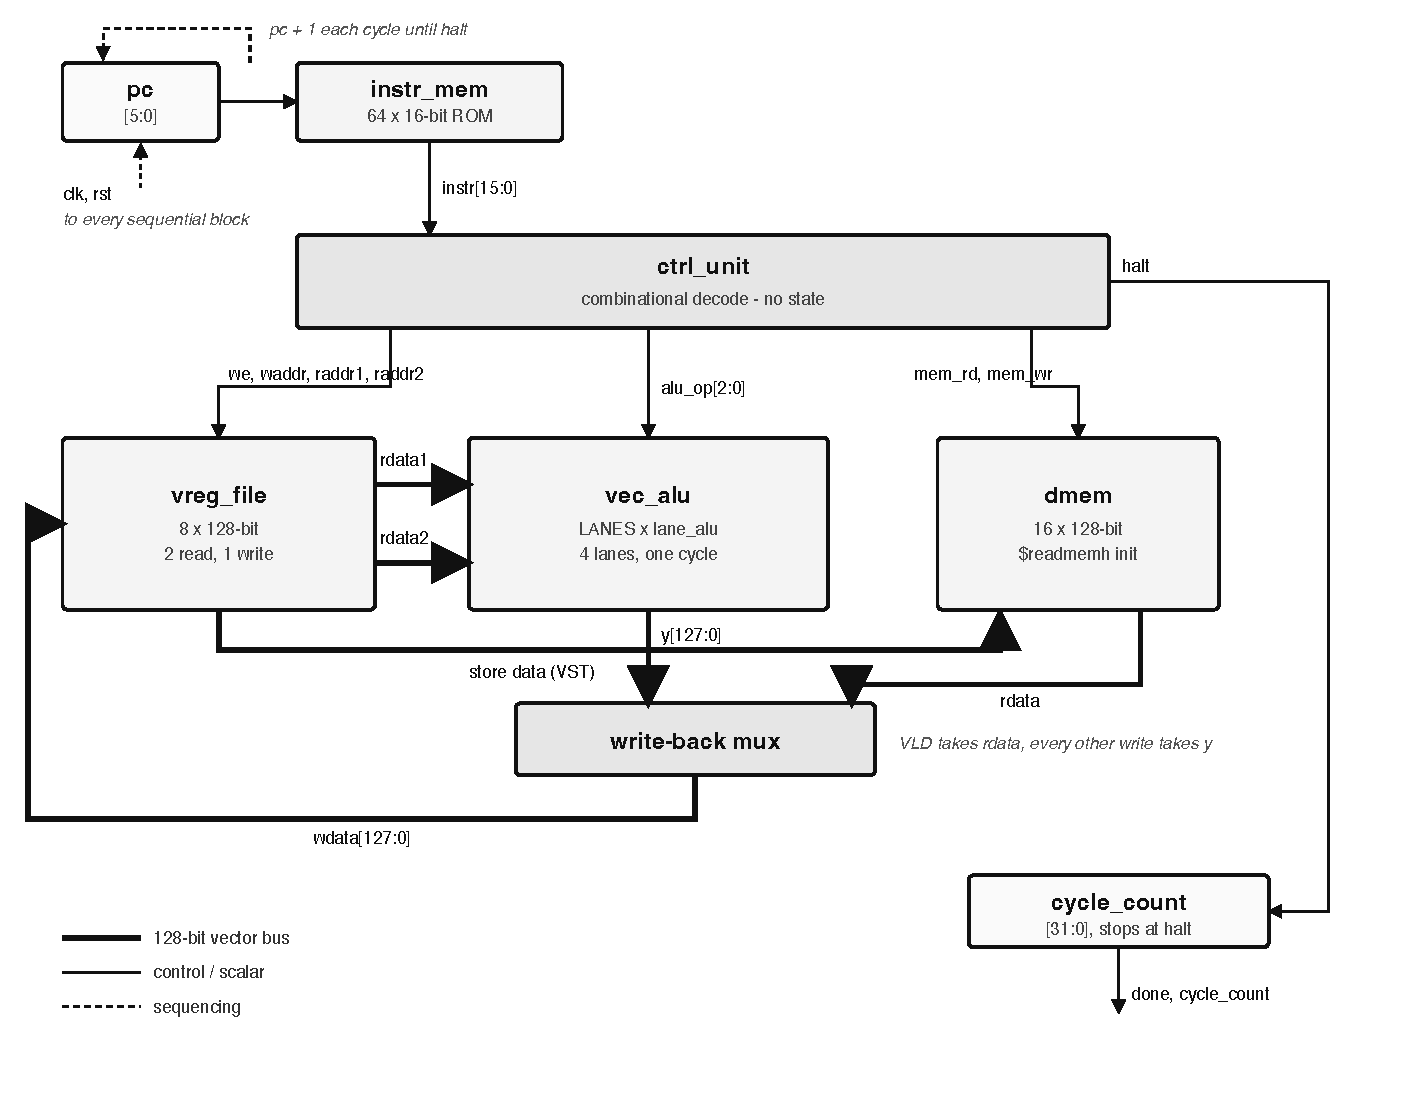
\includegraphics[width=\columnwidth]{top_level.pdf}
\caption{Vector processor datapath showing fetch, decode, ALU, memory,
and register write-back.}
\label{fig:architecture}
\end{figure}

\subsection{Instruction Format and Control}
Compute instructions encode the opcode in bits 15--12, destination in
11--9, first source in 8--6, and second source in 5--3. The low three bits
are unused for compute instructions. Both memory operations use bits 3--0
as a word address. Loads write \texttt{vd}. Stores take their data from
\texttt{vs1} through the first register read port.

The combinational decoder uses fixed slices for the register addresses and
an explicit case statement for operation and enable signals. Compute
instructions set the register write enable and select an ALU operation.
\texttt{VLD} selects data memory on the write-back multiplexer and enables
the destination register. \texttt{VST} enables the memory write. The
undefined opcodes advance the PC without modifying the register file or
data memory. At the clock edge for HALT, the top-level controller asserts
\texttt{done} and holds the PC and cycle count. The register-file and
data-memory write enables are gated during reset and after completion.

\subsection{Vector Execution}
Each lane consumes one 32-bit slice from each input, with lane 0 in the
least significant 32 bits. The four lanes share an operation code and
compute independently. Addition and subtraction wrap modulo $2^{32}$ per
lane. Bitwise operations include AND and OR. Equality and signed less-than
return a lane value of zero or one. Shift-left uses the low five bits of
the second operand as the shift distance.

\subsection{Scalar Baseline and Evaluation Method}
The scalar baseline uses a single instance of the same 32-bit ALU. For each
element, it loads A, loads B, adds, and stores, using one cycle per step.
The SIMD program performs the corresponding four steps per group of four
elements, with the loop unrolled. The scalar index advances during the
store cycle. The two cores use the same input values in scalar and vector
memory layouts. Both counters exclude reset and the terminal halt step. The SIMD machine
counts undefined opcodes as ordinary cycles.

\section{Results and Discussion}
\label{sec:evaluation}
\subsection{Array Addition and Logic Benchmarks}
Table~\ref{tab:cycles} gives the Icarus Verilog simulation results
\cite{icarus}. For sixteen elements, the vector program processes four
groups in 16 counted cycles. The scalar baseline takes 64 cycles. Fourfold
cycle-count improvement follows from keeping all four lanes occupied and
moving one full vector per load or store. End-to-end throughput in
elements per second also depends on the clock periods. The design has no
masking or vector-length control for a partially full final group.

\begin{table}[t]
\centering
\caption{Simulation results for 16-element array addition}
\label{tab:cycles}
\begin{tabular}{@{}lrrr@{}}
\toprule
Design & Lanes & Cycles & Elements/cycle \\
\midrule
Scalar & 1 & 64 & 0.25 \\
SIMD & 4 & 16 & 1.00 \\
\bottomrule
\end{tabular}
\end{table}

\subsection{Waveforms and Verification}
All eight RTL testbenches passed. The decoder passed 13 directed checks.
The integration suite passed 15 checks across the load--add--store demo,
array addition, and logic and comparison programs, which took 4, 16, and
10 counted cycles respectively. The system test passed 18 checks, including
result words, cycle counts, and preservation of array-add inputs.
Fig.~\ref{fig:lanes} records lane-level activity. Fig.~\ref{fig:system}
shows the top-level benchmark trace.

\begin{figure}[t]
\centering
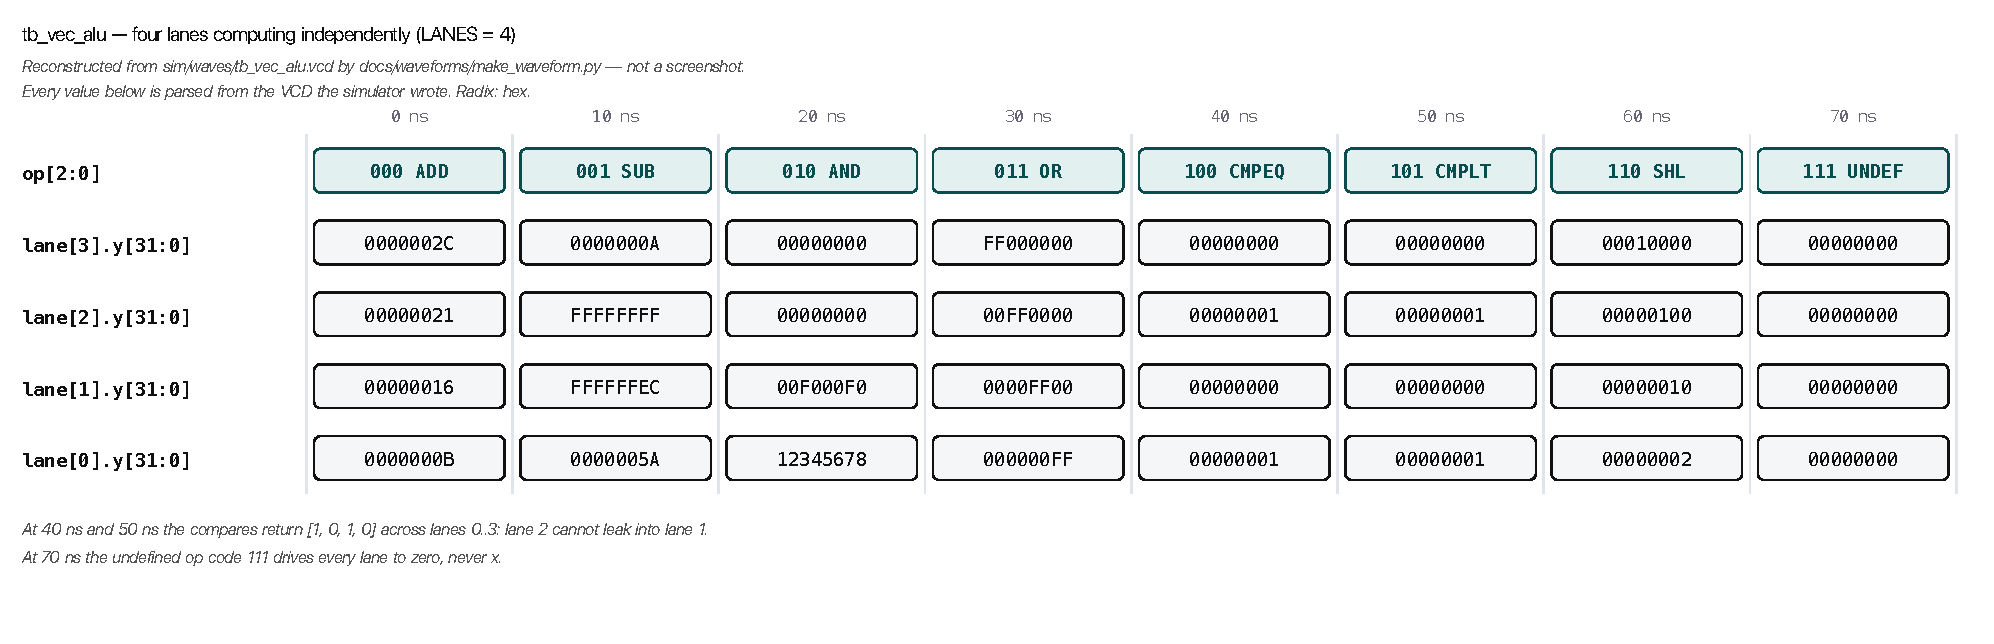
\includegraphics[width=\columnwidth]{vec_alu.pdf}
\caption{Vector ALU timing reconstructed from the simulation VCD.
The four lanes produce distinct outputs concurrently.}
\label{fig:lanes}
\end{figure}

\begin{figure*}[t]
\centering
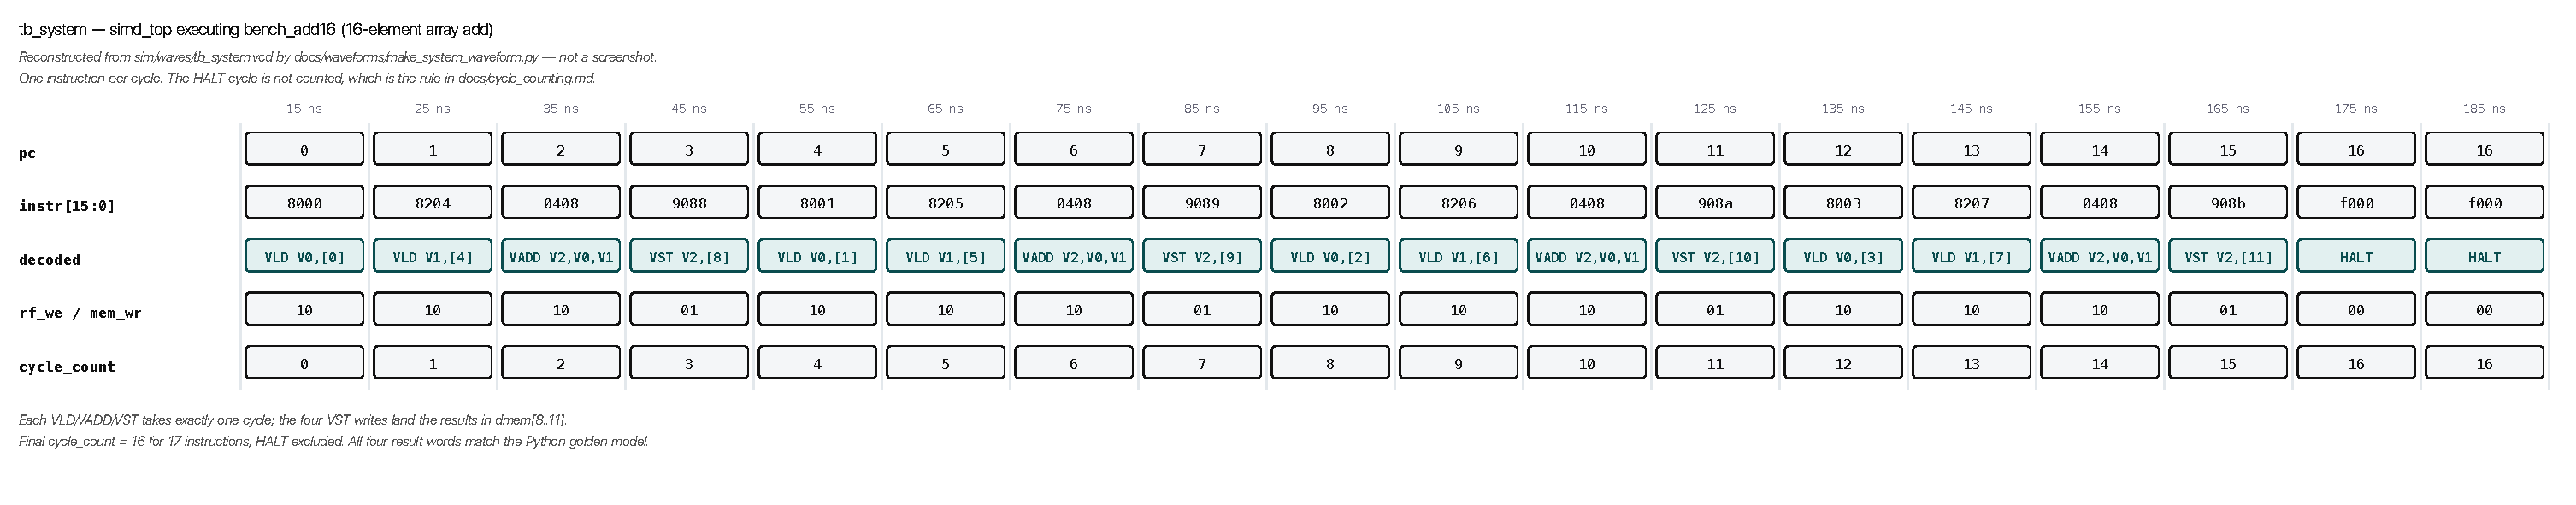
\includegraphics[width=0.98\textwidth]{system_pass.pdf}
\caption{System simulation trace reconstructed from the VCD. The PC and
instruction fields track the load--load--add--store groups. The counter
holds at 16 when \texttt{done} asserts.}
\label{fig:system}
\end{figure*}

A separate regression ran 2,000 generated programs with seed 7. The RTL
and the independent Python ISA simulator agreed on final memory and
cycle counts for all programs. Randomizing the first instruction exposed
a reset-time write defect that directed tests beginning with a vector load
had missed. The write-enable gates resolved the defect. The regression
covers four lanes and reset at startup. Mid-program reset and eight-lane
end-to-end execution remain outside that regression.

\subsection{Synthesis and Limitations}
Yosys mapped the ALU modules to Xilinx primitives \cite{yosys}.
The single-lane ALU used 251 LUTs and 19 CARRY4 primitives. The four-lane
ALU used 1,012 LUTs and 76 CARRY4 primitives, equivalent to
$4.03\times$ the LUT count and $4.00\times$ the carry resources.
The fixed instruction program allowed the synthesis flow to optimize
away much of the integrated core, so its cell count is excluded from the
area comparison. The flow performed no device-level placement, routing,
or timing analysis. A runtime-loadable instruction memory and a
device-targeted flow would enable a whole-core area and timing comparison.

\section{Individual Contributions}
\begin{itemize}
\item \textbf{Shaik Tajuddin} developed the Python golden model, ISA fuzzer,
system testbench, build and CI integration, and synthesis tooling. He also
prepared verification evidence and assembled the Phase I report.
\item \textbf{Parthraj Singh Bhati} froze the ISA and interfaces, implemented
the control unit and instruction ROM, integrated the SIMD core, and wrote
the decoder and integration testbenches and architecture write-up.
\item \textbf{Himanshu Pandey} implemented the lane ALU and vector ALU,
wrote their testbenches, and documented lane replication and the datapath.
\item \textbf{Jivit Rana} implemented and tested the scalar baseline,
worked on the benchmark programs, and documented the cycle-counting
method and performance comparison.
\item \textbf{Satya Yadav} implemented and tested the vector register
file and data memory and contributed register-file verification and report
updates.
\end{itemize}

\section{Conclusion}
The four-lane SIMD core executes the supported instruction set in
simulation and achieves four times the element throughput per counted
cycle of the scalar baseline on the 16-element addition. The directed
tests, system comparison, and randomized regression provide evidence for
functional correctness within their tested scope. Module-level synthesis
shows the hardware cost of replicating the ALU. Broader workloads,
partial-vector handling, and device-level timing would extend the
evaluation beyond this benchmark.

\newpage
\bibliographystyle{IEEEtran}
\bibliography{../docs/refs}

\end{document}
